% =============================================================================
% CHAPITRE 4 — RÉALISATION ET PRÉSENTATION DE L'APPLICATION DROPPY
% =============================================================================

\chapter{Réalisation et présentation de l'application Droppy}

% =============================================================================
% 4.1 INTRODUCTION
% =============================================================================

\section{Introduction}

Après avoir présenté les besoins et la conception de la solution, ce chapitre
est consacré à la présentation de l'application Droppy réalisée.

L'objectif est de présenter les principales interfaces de la solution ainsi
que les fonctionnalités accessibles à travers le dashboard. Les différentes
captures d'écran permettent d'illustrer concrètement le résultat obtenu et
le parcours d'utilisation de l'application.


% =============================================================================
% 4.2 PRÉSENTATION GÉNÉRALE DE L'APPLICATION
% =============================================================================

\section{Présentation générale de l'application}

\subsection{Écran principal}

L'écran principal constitue le point d'entrée de l'application. Il offre une
vue synthétique des informations importantes et permet à l'utilisateur
d'accéder rapidement aux différentes fonctionnalités de supervision.

\begin{figure}[H]
    \centering
    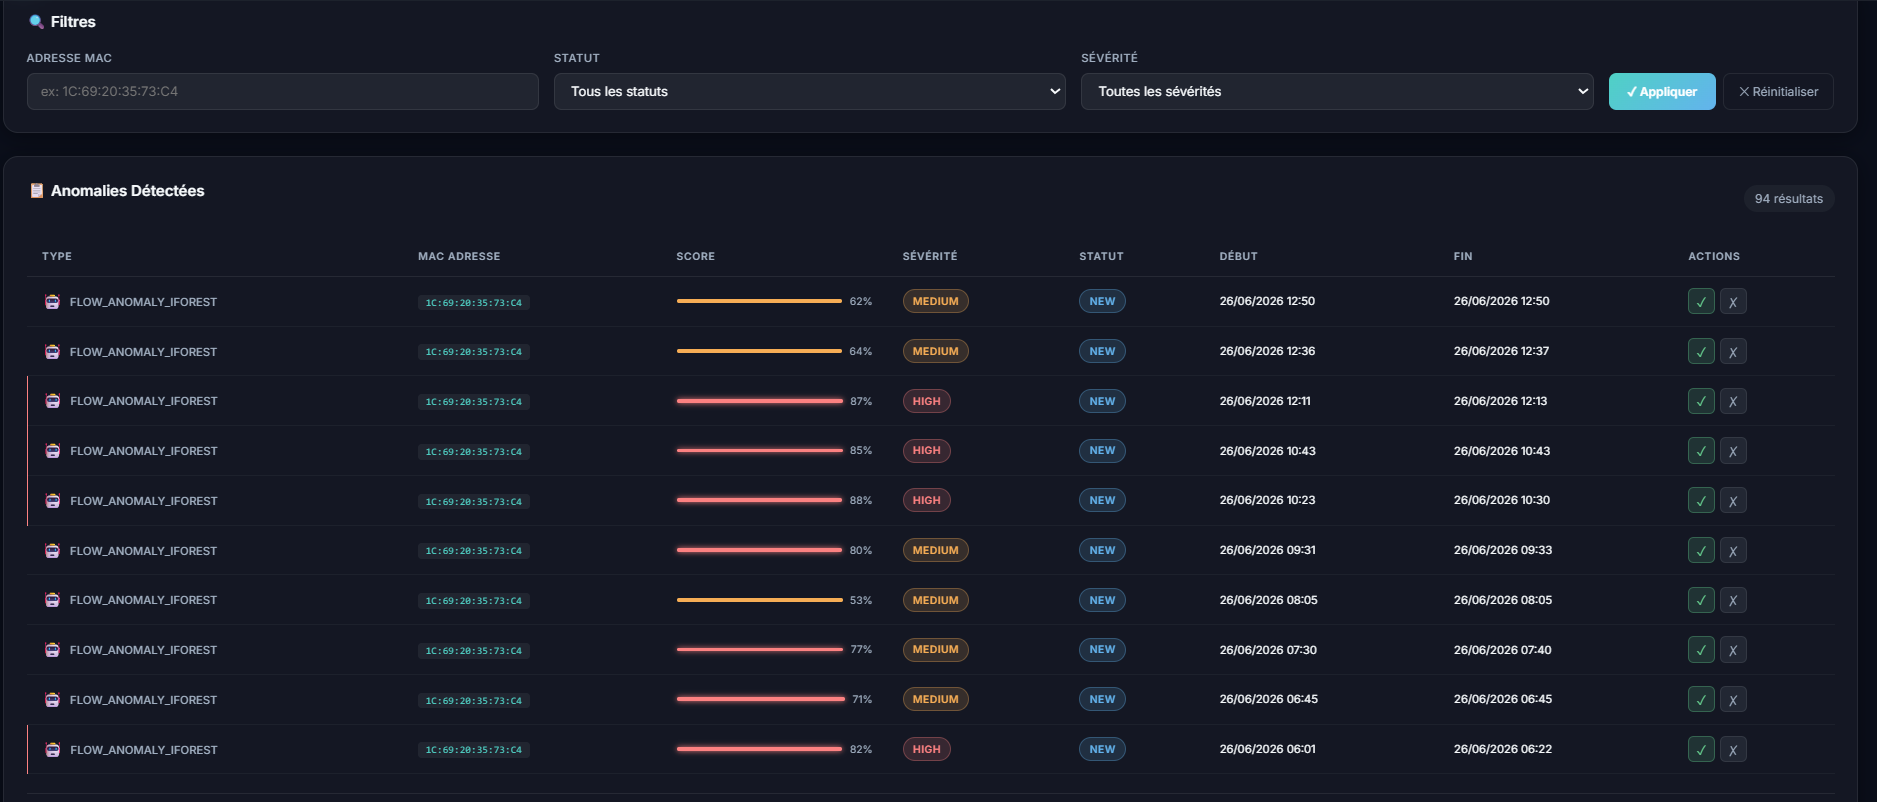
\includegraphics[width=\textwidth]{images/real.png}
    \caption{Écran principal du dashboard Droppy}
    \label{fig:dashboard}
\end{figure}


\subsection{Organisation de l'interface}

L'interface a été conçue afin de regrouper les informations essentielles dans
une présentation claire et directement exploitable par l'utilisateur.

\begin{figure}[H]
    \centering
    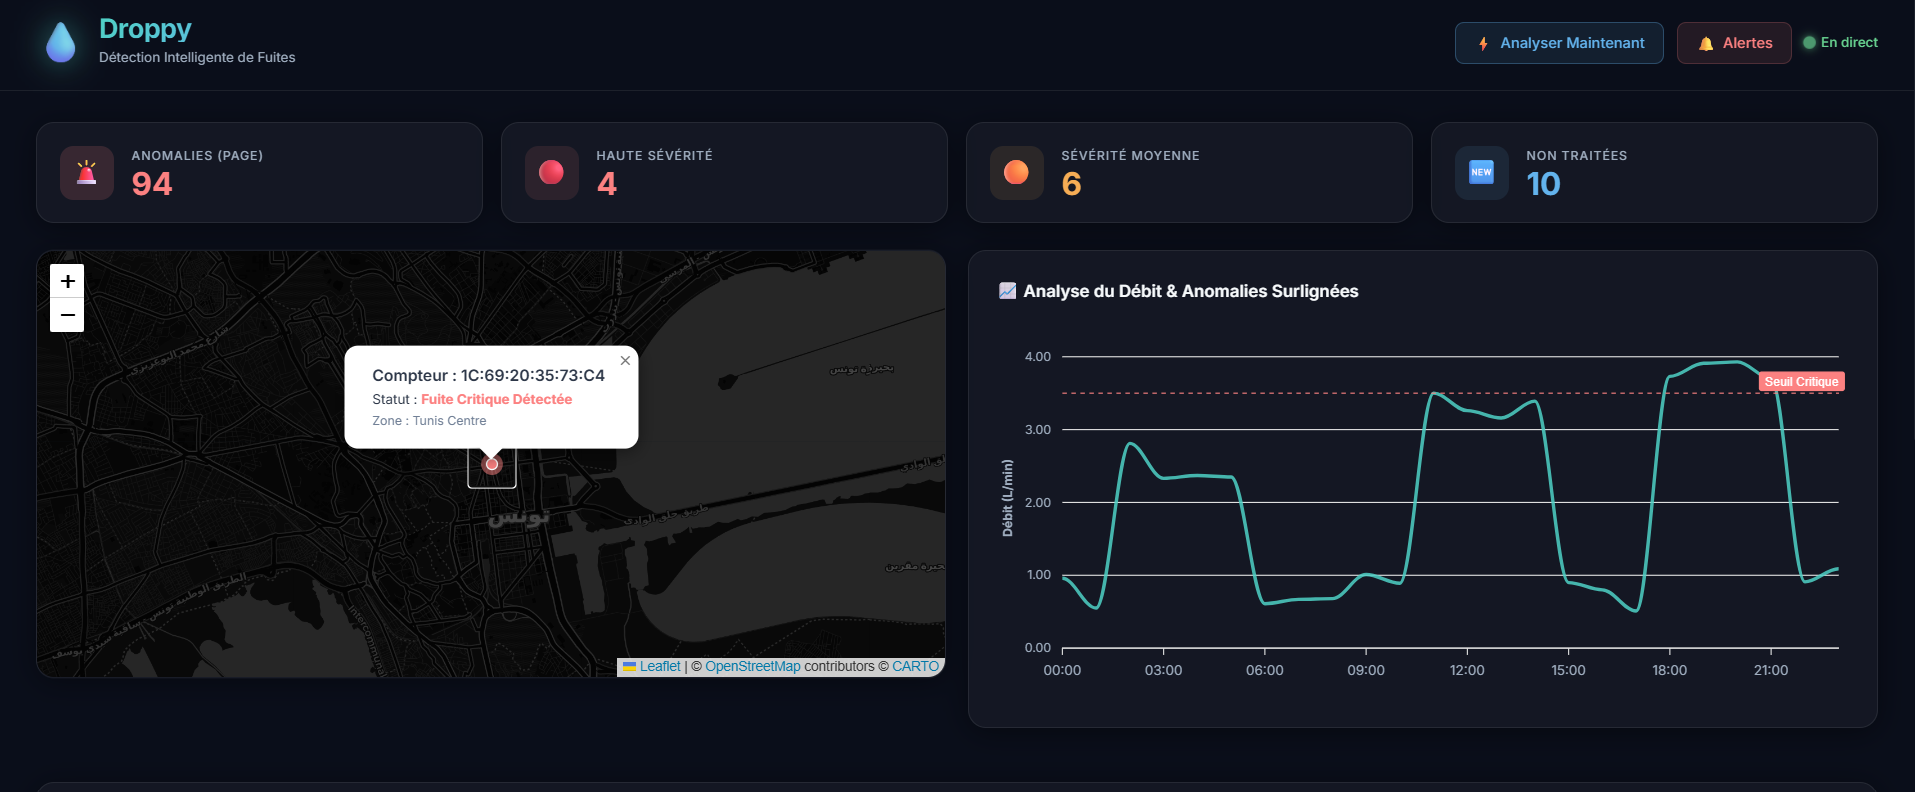
\includegraphics[width=\textwidth]{images/real2.png}
    \caption{Organisation générale de l'interface}
    \label{fig:interface-generale}
\end{figure}


% =============================================================================
% 4.3 SUPERVISION DES ANOMALIES
% =============================================================================

\section{Visualisation des données}

\subsection{Graphiques de suivi}

Les graphiques permettent de visualiser l'évolution des données et de
faciliter l'interprétation des différents événements observés.

\begin{figure}[H]
    \centering
    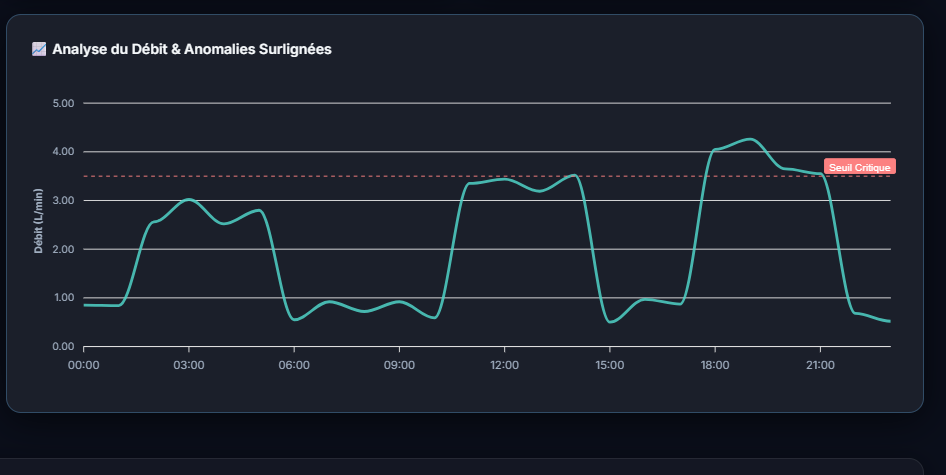
\includegraphics[width=\textwidth]{images/analyse.png}
    \caption{Visualisation graphique des données}
    \label{fig:graphiques}
\end{figure}



\subsection{Visualisation cartographique}

La carte permet de localiser les événements associés aux dispositifs
supervisés et d'offrir une représentation géographique des anomalies.

\begin{figure}[H]
    \centering
    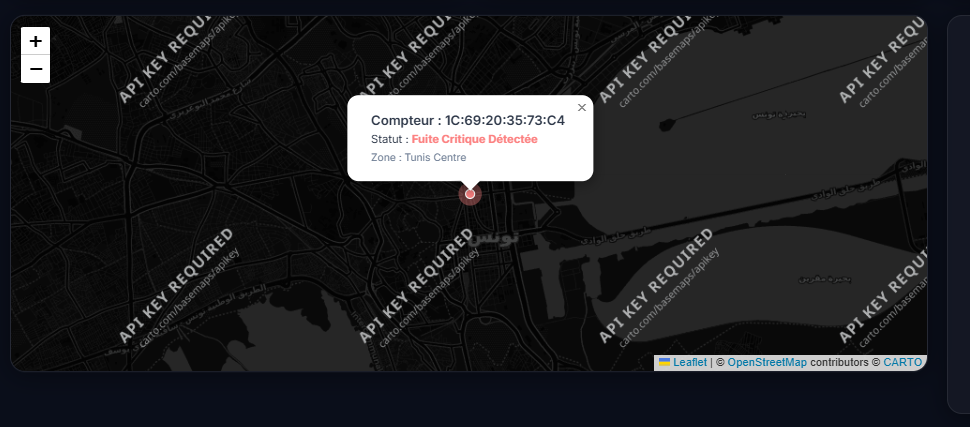
\includegraphics[width=\textwidth]{images/carteographie.png}
    \caption{Visualisation cartographique des anomalies}
    \label{fig:carte}
\end{figure}


% =============================================================================
% 4.5 ANALYSE INTELLIGENTE
% =============================================================================

\section{Analyse intelligente}
\subsection{Déclenchement d'une analyse}
L'utilisateur peut lancer une analyse depuis l'interface afin d'obtenir une
évaluation de l'état d'un dispositif.

\begin{figure}[H]
    \centering
    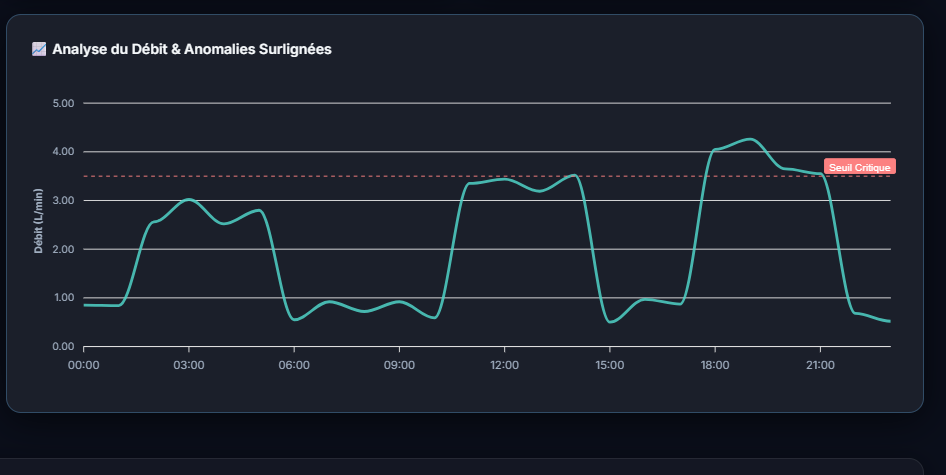
\includegraphics[width=\textwidth]{images/analyse.png}
    \caption{Déclenchement d'une analyse}
    \label{fig:analyse}
\end{figure}


\section{Conclusion}

Ce chapitre a présenté la réalisation de l'application Droppy à travers ses
principales interfaces et fonctionnalités.

Les différentes captures permettent d'illustrer concrètement le résultat
final de la solution, depuis la supervision générale jusqu'à la consultation
des anomalies, la visualisation des données, l'analyse et la prévision.

Le chapitre suivant sera consacré aux tests et à la validation de la solution.